% PGFPlots matrix plot generated from numpy array
% Matrix size: 7x7
% Data range: [0.000000, 1.000000]

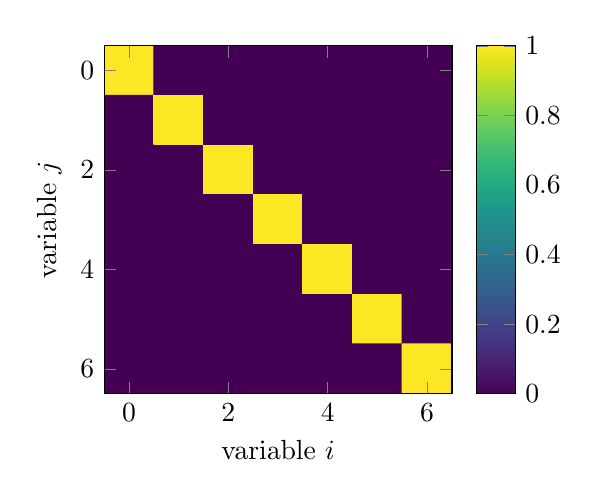
\begin{tikzpicture}
\begin{axis}[
    width=8cm,
    height=6cm,
    enlargelimits=false,
    axis equal image,
    colormap/viridis,
    xmin=-0.5, xmax=6.5,
    ymin=-0.5, ymax=6.5,
    colorbar,
    xlabel={variable $i$},
    ylabel={variable $j$}
]

\addplot[
    matrix plot,
    mesh/cols=7,
    point meta=explicit
] table[meta=z] {
x y z
0 0 1.000000
1 0 0.000000
2 0 0.000000
3 0 0.000000
4 0 0.000000
5 0 0.000000
6 0 0.000000
0 1 0.000000
1 1 1.000000
2 1 0.000000
3 1 0.000000
4 1 0.000000
5 1 0.000000
6 1 0.000000
0 2 0.000000
1 2 0.000000
2 2 1.000000
3 2 0.000000
4 2 0.000000
5 2 0.000000
6 2 0.000000
0 3 0.000000
1 3 0.000000
2 3 0.000000
3 3 1.000000
4 3 0.000000
5 3 0.000000
6 3 0.000000
0 4 0.000000
1 4 0.000000
2 4 0.000000
3 4 0.000000
4 4 1.000000
5 4 0.000000
6 4 0.000000
0 5 0.000000
1 5 0.000000
2 5 0.000000
3 5 0.000000
4 5 0.000000
5 5 1.000000
6 5 0.000000
0 6 0.000000
1 6 0.000000
2 6 0.000000
3 6 0.000000
4 6 0.000000
5 6 0.000000
6 6 1.000000
};

\end{axis}
\end{tikzpicture}
